%me=0 student solutions (ps file), me=1 - my solutions (sol file), me=2 - assignment (hw file)
\def\me{0}
\def\num{4}  %homework number
\def\due{Tuesday, October 6}  %due date
\def\course{CSCI-GA.1170-001/002 Fundamental Algorithms} %course name, changed only once
\def\name{GOWTHAM GOLI (N17656180)}   %student changes (instructor keeps!)
%
\iffalse
INSTRUCTIONS: replace # by the homework number.
(if this is not ps#.tex, use the right file name)

  Clip out the ********* INSERT HERE ********* bits below and insert
appropriate TeX code.  Once you are done with your file, run

  ``latex ps#.tex''

from a UNIX prompt.  If your LaTeX code is clean, the latex will exit
back to a prompt.  To see intermediate results, type

  ``xdvi ps#.dvi'' (from UNIX prompt)
  ``yap ps#.dvi'' (if using MikTex in Windows)

after compilation. Once you are done, run

  ``dvips ps#.dvi''

which should print your file to the nearest printer.  There will be
residual files called ps#.log, ps#.aux, and ps#.dvi.  All these can be
deleted, but do not delete ps1.tex. To generate postscript file ps#.ps,
run

  ``dvips -o ps#.ps ps#.dvi''

I assume you know how to print .ps files (``lpr -Pprinter ps#.ps'')
\fi
%
\documentclass[11pt]{article}
\usepackage{amsfonts}
\usepackage{latexsym}
\usepackage[lined,boxed,linesnumbered]{algorithm2e}
\usepackage{amsmath}
\usepackage{amsthm}
\usepackage{array}
\usepackage{amssymb}
\usepackage{amsthm}
\usepackage{epsfig}
\usepackage{psfrag}
\usepackage{color}
\usepackage{tikz}
\usepackage{enumerate}
\usetikzlibrary{calc,trees,positioning,arrows,fit,shapes,calc}
\usetikzlibrary{trees}
\usepackage{mathtools}
\usepackage{float}
\setlength{\oddsidemargin}{.0in}
\setlength{\evensidemargin}{.0in}
\setlength{\textwidth}{6.5in}
\setlength{\topmargin}{-0.4in}
\setlength{\textheight}{8.5in}
\newtheorem{theorem}{Theorem}
\newcommand{\handout}[5]{
   \renewcommand{\thepage}{#1, Page \arabic{page}}
   \noindent
   \begin{center}
   \framebox{
      \vbox{
    \hbox to 5.78in { {\bf \course} \hfill #2 }
       \vspace{4mm}
       \hbox to 5.78in { {\Large \hfill #5  \hfill} }
       \vspace{2mm}
       \hbox to 5.78in { {\it #3 \hfill #4} }
      }
   }
   \end{center}
   \vspace*{4mm}
}
\definecolor{myblue}{RGB}{56,94,141}
\newcounter{pppp}
\newcommand{\prob}{\arabic{pppp}}  %problem number
\newcommand{\increase}{\addtocounter{pppp}{1}}  %problem number

%first argument desription, second number of points
\newcommand{\newproblem}[2]{
\ifnum\me=0
\ifnum\prob>0 \newpage \fi
\increase
\setcounter{page}{1}
\handout{\name, Homework \num, Problem \arabic{pppp}}{\today}{Name: \name}{Due:
\due}{Solutions to Problem \prob\ of Homework \num\ (#2)}
\else
\increase
\section*{Problem \num-\prob~(#1) \hfill {#2}}
\fi
}

%\newcommand{\newproblem}[2]{\increase
%\section*{Problem \num-\prob~(#1) \hfill {#2}}
%}

\def\squarebox#1{\hbox to #1{\hfill\vbox to #1{\vfill}}}
\def\qed{\hspace*{\fill}
        \vbox{\hrule\hbox{\vrule\squarebox{.667em}\vrule}\hrule}}
\newenvironment{solution}{\begin{trivlist}\item[]{\bf Solution:}}
                      {\qed \end{trivlist}}
\newenvironment{solsketch}{\begin{trivlist}\item[]{\bf Solution Sketch:}}
                      {\qed \end{trivlist}}
\newenvironment{code}{\begin{tabbing}
12345\=12345\=12345\=12345\=12345\=12345\=12345\=12345\= \kill }
{\end{tabbing}}

%\newcommand{\eqref}[1]{Equation~(\ref{eq:#1})}

\newcommand{\hint}[1]{({\bf Hint}: {#1})}
%Put more macros here, as needed.
\newcommand{\room}{\medskip\ni}
\newcommand{\brak}[1]{\langle #1 \rangle}
\newcommand{\bit}[1]{\{0,1\}^{#1}}
\newcommand{\zo}{\{0,1\}}
\newcommand{\C}{{\cal C}}

\newcommand{\nin}{\not\in}
\newcommand{\set}[1]{\{#1\}}
\renewcommand{\ni}{\noindent}
\renewcommand{\gets}{\leftarrow}
\renewcommand{\to}{\rightarrow}
\newcommand{\assign}{:=}

\newcommand{\AND}{\wedge}
\newcommand{\OR}{\vee}

\newcommand{\Forr}{\mbox{\bf For }}
\newcommand{\To}{\mbox{\bf to }}
\newcommand{\Do}{\mbox{\bf Do }}
\newcommand{\Ifi}{\mbox{\bf If }}
\newcommand{\Thenn}{\mbox{\bf Then }}
\newcommand{\Elsee}{\mbox{\bf Else }}
\newcommand{\Whilee}{\mbox{\bf While }}
\newcommand{\Repeatt}{\mbox{\bf Repeat }}
\newcommand{\Until}{\mbox{\bf Until }}
\newcommand{\Returnn}{\mbox{\bf Return }}
\newcommand{\Swap}{\mbox{\bf Swap }}

\begin{document}

\ifnum\me=0
%\handout{PS\num}{\today}{Name: **** INSERT YOU NAME HERE ****}{Due:
%\due}{Solutions to Problem Set \num}
%
%I collaborated with *********** INSERT COLLABORATORS HERE (INDICATING
%SPECIFIC PROBLEMS) *************.
\fi
\ifnum\me=1
\handout{PS\num}{\today}{Name: Yevgeniy Dodis}{Due: \due}{Solution
{\em Sketches} to Problem Set \num}
\fi
\ifnum\me=2
\handout{PS\num}{\today}{Lecturer: Yevgeniy Dodis}{Due: \due}{Problem
Set \num}
\fi





\newproblem{Fast $k$-way Merging}{10 points}

Using a min-heap in a clever way, give $O(n\log k)$-time algorithm to
merge $k$ sorted arrays $A_1\ldots A_k$ of size $n/k$ each into one
sorted array $B$.  Write the pseudocode of your algorithm using
procedures {\sc Build-Heap}, {\sc Extract-Min} and {\sc Insert}.

\ifnum\me<2
\begin{solution}

\section*{Algorithm}
\begin{itemize}
\item Build a Heap using the first elements of the given arrays $A_1, \ldots, A_k$
\item Extract Minimum from the heap and insert into $B$
\item Pick the next element from the array, the popped element of the heap came from and insert into this heap
\item Keep repeating until all the elements of the given arrays are inserted into the heap
\end{itemize}

\section*{Psuedocode}

\IncMargin{1em}
\begin{algorithm}[H]
\TitleOfAlgo{{\sc MergeHeaps}($A_1,\ldots,A_k, B$)}
$Heap$ $\leftarrow$ {\sc Build-Heap}($A_1[0],\ldots,A_k[0]$)\\
$B \leftarrow$ {\sc newArray}(n)\\
$c$ $\leftarrow$ 0\\
\While{Heap is not empty}{
	$A_i[p]$ $\leftarrow$ = {\sc Extract-Min}($Heap$)\\
	$B[c]$ $\leftarrow$ $A_i[p]$\\
	\If{p $<$ n/k}{
		{\sc Insert}$(A[p+1], Heap)$\\
	}
	$c$$++$
}
\Returnn $B$
\caption{Merge sorted arrays $A_1,\ldots,A_k$ using a min-heap}
\end{algorithm}
\pagebreak
\section*{Time Complexity}
In the first step, time taken to build heap of size $k$ is $O(k)$. 
Time taken to extract minimum from the heap and then insert into the heap is $O(\log k)$ and this is done $n$ times, therefore $O(n\log k)$
Therefore, total time takes is $O(k) + O(n\log k) = O(n\log k)$

\end{solution}
\fi



\newproblem{Finding a Repetitor}{26 (+14) Points}

Your are given an array $A[1]\ldots A[n]$ of $n$ ``objects''. You
have a magic unit-time procedure $Equal(A[i],A[j])$, which will tell
if objects $A[i]$ and $A[j]$ are the same.
%(This test is naturally assumed to be commutative and associative,
%so no surprises there.)
Unfortunately, there is no other way to get any meaningful
information about the objects: e.g., cannot ask if $A[i]$ is
``greater'' than $A[j]$ of if it is more ``sexy'', etc., just the
equality test.  We say that $A$ is a {\em repetitor} if it contains
strictly more than $n/2$ elements which are all pairwise the same.
In this case any of $A$'s (at least $n/2$) repetitive elements is
called {\em dull}. For example, if the ``object'' is a string, the
array $(boring, funny, cute, boring, boring)$ is a repetitor where
$boring$ is dull while $funny$ is not. On the other hand, the array
$(hello, hi, bonjorno, hola, whasup)$ is not a repetitor.  You goal
is to determine if $A$ is a repetitor, and, if so, output its dull
``object'' (which is clearly unique).

\begin{itemize}

\item[(a)] (8 points) Design a simple divide-and-conquer algorithm for this
problem running in time $O(n\log n)$. Make sure you argue the
correctness and the running time.\\
\hint{Prove that if $A$ is a repetitor, at least one of its
``halves'' is as well.}

\ifnum\me<2
\begin{solution}
\begin{theorem}
If $A$ is a repetitor, at least one of its
``halves'' is as well
\end{theorem}
\begin{proof}

Let $p$ be the dull of $A$. 
If the left half of $A$ is not a repetitor then there are less than $n/4$ occurrences of $p$  in $A[1 \ldots mid]$ which implies that the right half $A[mid+1 \ldots n]$ has to have more than $n/4$ occurrences of $p$ for $p$ to be a dull of $A$. Therefore, the right half is a repetitor. Similarly, we can argue for the left half to be a repetitor. 

If neither of the halves of $A$ is a repetitor, it means that there are less than $n/4$ occurrences of $p$  in $A[1 \ldots mid]$ and  $A[mid+1 \ldots n]$. Therefore, $p$ cannot be the dull in this case

If both the halves of $A$ are repetitors then $A[1 \ldots mid]$ has to have more than $n/4$ occurrences of $p$ and  $A[mid+1 \ldots n]$ has to have more than $n/4$ occurrences of $p$ for $p$ to be a dull of $A$.

Therefore we can conclude that If $A$ is a repetitor, at least one of its
``halves'' is as well 
\end{proof}
Using the above theorem, we can implement a $O(n \log n)$ algorithm as follows

\section*{Psuedocode}
\IncMargin{1em}
\begin{algorithm}[H]
\TitleOfAlgo{{\sc FindDull}(A, low, high)}
\If{low is high}{
\textbf{return} $A[low]$
}
\Else{
	$mid$ $\leftarrow$ (low + high)/2\\
	$leftDull$ $\leftarrow$ {\sc FindDull}($A, low, mid$)\\
	$rightDull$ $\leftarrow$ {\sc FindDull}($A, mid+1, high$)\\
	\If{leftDull is rightDull}{
		\Returnn $leftDull$
	}
	
	\Else{
		$lDullCount$ = {\sc CountOccurrences}($leftDull, A[low \ldots high$])\\
		$rDullCOunt$ = {\sc CountOccurrences}($rightDull, A[low \ldots high$])\\
		
		\uIf{lDullCount $>$ (high - low)/2}{
			\Returnn$ leftDull$
		}
		\uElseIf{rDullCount $>$ (high - low)/2}{
			\Returnn $rightDull$
		}	
		\uElse{
			\Returnn {\sc NoDull}
		}
	}
}

\caption{Alorithm to find the dull OF $A$ in $O(n \log n)$ time}
\end{algorithm}

\end{solution}
\fi

\item[(b)] (4 Points) Remember, if $A$ was an integer array, the
procedure {\sc Partition}$(A,p,r)$ (see Section 7.1) makes $x=A[r]$
the pivot element and returns the index $q$, where the new value of
$A[q]$ contains the pivot $x$, the new values $A[p\ldots q-1]$
contain elements less or equal to $x$, and the new values
$A[q+1\ldots r]$ contain values greater than $x$. Write the
pseudocode of the modified procedure {\sc New-Partition}$(A,p,r)$,
which only uses the $Equal$ operator and returns $q$ such that
$A[q+1\ldots r]$ contain all the elements equal to $x$ (while
$A[p\ldots q]$ contain all other elements).

\ifnum\me<2
\begin{solution}
\section*{Psuedocode}
\IncMargin{1em}
\begin{algorithm}[H]
\TitleOfAlgo{{\sc New-Partition}$(A,p,r)$}
$x \leftarrow A[r]$\\
$i \leftarrow p-1$\\
\For{j = p to r-1}{
	\If{A[j] {\sc Not Equal} x}{
		$i \leftarrow i+1$\\
		{\sc Swap}($A[i], A[j])$\\
	}
}
{\sc Swap}($A[i+1], A[r])$\\
\Returnn $i+1$
\caption{Modified procedure {\sc New-Partition}$(A,p,r)$ }
\end{algorithm}

\end{solution}
\fi

\item[(c)] (2 points) Consider the following, more general, algorithm
{\sc Repeat}$(A,n,t)$, which tells if some element of $A[1]\ldots
A[n]$ is repeated at least $t$ times. (Clearly, {\sc Repetitor} can
just call {\sc Repeat} with $t=n/2+1$.)

\begin{code}
{\sc Repeat}$(A,~n,~t)$\\
\> \Ifi $n<t$ \Returnn $no$\\
\> Pick $i\in \{1\ldots n\}$ {\em at random}.\\
\> $Swap(A[i],A[n])$\\
\> $q\leftarrow${\sc New-Partition}$(A,~1,~n)$\\
\> \Ifi $n-q\ge t$ \Thenn \Returnn $(yes,A[n])$ \\
\> \Returnn {\sc Repeat}$(A,~q,~t)$
\end{code}

Argue that the algorithm above is correct.

\ifnum\me<2
\begin{solution}

It is quite obvious that $t \leq n$, Therefore if $t > n$ the algorithm returns \textit{no}

Let the randomly picked element be $key$. {\sc New-Partition}$(A, 1, n)$ returns $A$ such that $A[1 \ldots q-1] \neq key$ and $A[q \ldots n] = key$. Therefore the array has $n-q$ occurrences of $key$

If $n-q \geq t$ then $key$ is repeated atleast $t$ times. Else we keep repeating the procedure with a new key each time until we find an element that is repeated atleast t times
\end{solution}
\fi

\item[(d)] (3 points) Argue that the algorithm above
always terminates in time $O(n^2)$ (irrespective of the random
choices of $i$).

\ifnum\me<2
\begin{solution}
In the worst case scenario, If the array has all distinct elements and no element can occurs more than $t$ times ($ \because t \geq 2$), $q$ will be $n-1$ in the first recursive call, $n-2$ in the second recursive call, $n-3$ in the third recursive and so on until $1$ in the first recursive call

Therefore in the worst case, the running time $T(n)$ is
\begin{equation*}
\begin{split}
T(n) &= T(n-1) + n\\
&= T(n-2) + n-1 + n \\
&= T(n-3) + n-2 + n-1 + n\\
\vdots\\
&= 1 + 2 + \ldots +  n-1 + n\\
&= \frac{n(n+1)}{2}\\
&= O(n^2)\\
\end{split}
\end{equation*} 
\end{solution}
\fi

\item[(e)] (3 points) Give an example of an (integer) array $A$ and a
value $t\ge 2$ where the algorithm indeed takes time $\Omega(n^2)$.

\ifnum\me<2
\begin{solution}
Let $A = [1, 2, 3, 4, 5, 6, 7, 8, 9] $ and $t = 3$. There is no element in $A$ that occurs more than 3 times. The algorithm will run as follows

Irrespective of the element picked as the pivot, as all the elements are distinct, $q$ will be $n-1$ (i.e 8) in the first recursive call, $n-2$ (i.e 7) in the second recursive call and so on until $1$ in the first recursive call.

$\implies T(n) = 1 + 2 + \ldots + n = n(n+1)/2 = \Omega(n^2)$
\end{solution}
\fi

\item[(f)] (4 Points) Let $T(n)$ be the worst case (over all
arrays $A[1\ldots n]$ and $t>n/2$ such that $A$ contains $t$
identical elements) of the {\em expected} running time of {\sc
Repeat}$(A,n,t)$ (over the random choice of $i$). For concreteness,
assume {\sc New-Partition} takes time exactly $n$. Prove that
$$T(n) \le \frac{1}{2}\cdot T(n-1) + n$$
\hint{Prove that in this case no recursive sub-call will be made
with probability $t/n > 1/2$.}

\ifnum\me<2
\begin{solution}
Given that $A$ contains $t$ identical elements ($t > n/2$), Therefore $A$ is repititor and let $p$ be it's dull. 

If $p$ is randomly picked up as the pivot, then the algorithm will terminate after the first recursive call itself. Therefore the probability that there will be no recursive sub call is the (total number of occurrences of $p$)/(number of elements in A) $> (n/2n) = 1/2$

In the worst case, For a recursive call to happen, the pivot chosen has to be a unique non-dull (or the element with least number of repetitions if the elements are not distinct)  element of $A$. Probability that the  non-dull element will be chosen as a pivot is $< 1/2$

Therefore in the worst case of the expected running time, \\
$T(n)$ = (probability that the next recursive call will happen)(Time taken by the next recursive call) + $n$\\
$\implies T(n) \leq \frac{1}{2}. T(n-1) + n$
\end{solution}
\fi

\item[(g)] (2 points) Show by induction that $T(n)\le 2n$.

\ifnum\me<2
\begin{solution}

\textbf{Base case} - $T(1) = 1 \leq 2.1 = 2$. Base case is true

\textbf{Induction Hypothesis} - $T(k) \leq 2k, \,\,\, \forall k = 1, \ldots, n-1$

\textbf{Induction Step}
\begin{equation*}
\begin{split}
T(n) &\leq \frac{1}{2}. T(n-1) + n\\
&\leq \frac{1}{2} (2(n-1)) + n\\
&= n-1+n\\
&\leq 2n
\end{split}
\end{equation*}
By Induction, we can conclude that $T(n) \leq 2n$
\end{solution}
\fi

\item[(h$^{*}$)] ({\bf Extra Credit}; 6 points)
Consider the following test for repetitor. For 100 times, run {\sc
Repeat}$(A,n,n/2+1)$ for at most $4n$ steps. If one of these 100
runs ever finishes within $4n$ steps, use that answer. If none of
the $100$ runs terminates within $4n$ steps, return $no$. Argue that
the running time of this procedure is $O(n)$. Then argue that the
probability it returns the incorrect $no$ answer (when it should
have returned $yes$)
is at most $2^{-100}$.\\
\hint{Show that when the answer is $yes$, the probability of not
finding this answer in $4n$ steps is at most $1/2$. Google for
``Markov's inequality'' if you want to be formal.}

\ifnum\me<2
\begin{solution}
The test runs for at most $4n$ steps and 100 times, therefore total number of steps is $400n$. Therefore running time is $O(n)$ ($\because 400 << n$)
\end{solution}
\fi

\item[(i$^{**}$)] ({\bf Extra Credit}; 8 points)
Try to design $O(n)$ deterministic test for a repetitor.

\ifnum\me<2
\begin{solution}
\section*{\sc{Key Idea}}
The dull of the array remains preserved whenever we cancel a pair of distinct elements from the array
\section*{\sc{Psuedocode}}
\IncMargin{1em}
\begin{algorithm*}[H]
\TitleOfAlgo{{\sc Find-Dull}(A)}
$ count \leftarrow 0$\\
\For{i $\leftarrow$ 0 to n-1}{
	\uIf{count is 0}{
		$x \leftarrow A[i]$\\
		$count \leftarrow 1$\\
	}
	\uElseIf{x $\neq$ A[i]}{
		$count \leftarrow count - 1$\\
	}
	\Elsee{
		$count \leftarrow count+1$\\
	}
$num \leftarrow $ \sc{Count-Occurrences}($x,A$)\\
\uIf{num $>$ n/2}{
	\Returnn $x$
}
\uElse{
\Returnn NoDull
}
}
\caption{Algorithm to find dull of $A$ in $O(n)$ time}
\end{algorithm*}
To prove the correctness of the above algorithm it is sufficient if we prove that if $A$ is a repititor and say $\alpha$ is the dull then at the end of the for loop $x = \alpha$

In the above algorithm, during $i^{th}$ iteration, we compare $A[i-1]$ with $x$ and cancel both if they are different, and increment count otherwise.

So if $count=0$, then all elements upto $A[i-1]$ would have been eliminated through  distinct-elements pair formations. If $count >0$, then $\{x ,\ldots$ count times $\ldots ,x, A[i], \ldots A[n-1]\}$ elements would have still survived at the end of the $i^{th}$ iteration.\\ Let $S_i$ be  $\{x ,\ldots$ count times $\ldots ,x, A[i], \ldots A[n-1]\}$ then $\alpha$ is a dull of $S_i$.

At the end of for loop $S_n = \{x ,\ldots$ count times $\ldots ,x, A[n], \ldots A[n-1]\}$. It means that $\alpha$ is a dull of $\{x ,\ldots$ count times $\ldots ,x\}$
and $count > 0$. Hence $\alpha = x$
\end{solution}
\fi

\end{itemize}



\newproblem{Quicksort}{12 points}


Assume we are given an array $A[1\ldots n]$ of $n$ {\em distinct}
integers and that $n=2k$ is {\em even}.

\begin{itemize}

\item[(a)] (4 points) Let $pivot(A)$ denote the rank of the pivot
element at the end of the partition procedure, and assume that we
choose a random element $A[i]$ as a pivot, so that $pivot(A) = i$ with
probability $1/n$, for all $i$. Let $smallest(A)$ be the length of the
smaller sub-array in the two recursive subcalls of the {\sc
Quicksort}.  Notice, $smallest(A) = \min(pivot(A)-1,n-pivot(A))$ and
belongs to $\set{0\ldots k-1}$, since $n=2k$ is even. Given $0\le j\le
k-1$, what is the probability that $smallest(A)=j$?

\ifnum\me<2
\begin{solution}
Given that the probability to choose a random element $A[i]$ as a pivot is $1/n$. It is clear that there exists a pair $(A_i,A_j) \leq n$ such that $A[i]$ and $A[j]$ will result in the same \textit{smallest(A)} when chosen as a pivot. Therefore, there will be total $n/2$ pairs of $(A_i,A_j)$ that will result in the same \textit{smallest(A)} when chosen as a pivot which is illustrated in the figure below ($j_k$ denotes the case when $j = k$)
\begin{figure}[h]
 \centering
 \begin{tikzpicture}[ele/.style={fill=black,circle,minimum width=.8pt,inner sep=1pt},every fit/.style={ellipse,draw,inner sep=-2pt}]
  \node[ele,label=left:$A_1$] (a1) at (0,4) {};    
  \node[ele,label=left:$A_2$] (a2) at (0,3) {};    
  \node[ele,label=left:$\vdots$] (a3) at (0,2) {};
  \node[ele,label=left:$A_{n-1}$] (a4) at (0,1) {};
  \node[ele,label=left:$A_{n}$] (a5) at (0,0) {};
	
  \node[ele,,label=right:$j_1$] (b1) at (4,4) {};
  \node[ele,,label=right:$j_2$] (b2) at (4,3) {};
  \node[ele,,label=right:$\vdots$] (b3) at (4,2) {};
  \node[ele,,label=right:$j_{k-1}$] (b4) at (4,1) {};

  \node[draw,fit= (a1) (a2) (a3) (a4) (a5),minimum width=2.5cm] {} ;
  \node[draw,fit= (b1) (b2) (b3) (b4),minimum width=2.5cm] {} ;  
  \draw[->,thick,shorten <=2pt,shorten >=2pt] (a1) -- (b2);
  \draw[->,thick,shorten <=2pt,shorten >=2] (a2) -- (b1);
  \draw[->,thick,shorten <=2pt,shorten >=2] (a3) -- (b2);
  \draw[->,thick,shorten <=2pt,shorten >=2] (a3) -- (b4);
  \draw[->,thick,shorten <=2pt,shorten >=2] (a3) -- (b3);
  \draw[->,thick,shorten <=2pt,shorten >=2] (a3) -- (b1);
  \draw[->,thick,shorten <=2pt,shorten >=2] (a4) -- (b3);
  \draw[->,thick,shorten <=2pt,shorten >=2] (a5) -- (b4);
 \end{tikzpicture}
\end{figure}

As we know that the probability of selecting any $A_i$ as pivot is $1/n$. The probability that \textit{smallest}($A$)  will be $2/n$ (as two elements from the Pivot set point to one element in the Smallest set as seen above).
\begin{equation*}
\Pr(smallest(A) = j) = 2/n
\end{equation*}
\end{solution}
\fi

\item[(b)] (3 points) Compute the {\em expected value} of $smallest(A)$;
i.e., $\sum_{j=0}^{k-1} \Pr(smallest(A)=j)\cdot j$.\\
\hint{If you solve part (a) correctly, no big computation is needed
here.}

\ifnum\me<2
\begin{solution}
\begin{equation*}
\begin{split}
\sum_{j=0}^{k-1} \Pr(smallest(A)=j)\cdot j &= \sum_{j=0}^{k-1} 2/n.j\\
&= 2/n \sum_{j=0}^{k-1} j\\
&= \frac{2}{n} . \frac{k.(k-1)}{2}\\
&= \frac{n-2}{4}
\end{split}
\end{equation*}
\end{solution}
\fi

\item[(c)] (5 points) Write a recurrence equation for the running time $T(n)$
of {\sc Quicksort}, assuming that at every level of the recursion the
corresponding sub-arrays of $A$ are partitioned {\em exactly} in the
ratio you computed in part (b). Solve the resulting recurrence
equation. Is it still as good as the average case of randomized {\sc
Quicksort}?

\ifnum\me<2
\begin{solution}

For relatively large $n$ we can assume that $n-2/4 \approxeq n/4$. Therefore at every level of the recursion the array is partitioned into sub arrays of length $n/4$ and $3n/4$. 
\begin{equation*}
T(n) = T(n/4) + T(3n/4) + O(n)
\end{equation*}

This recurrence equation can be solved using Recursive tree method as shown below in the figure

\begin{figure}[H]
	\centering
	\includegraphics[width=0.95\columnwidth]{tree.jpg}
	\caption{Recursive Tree of $T(n)$}
	
\end{figure}
\begin{equation*}
\begin{split}
n \log_{4} n &\leq T(n) \leq n \log_{4/3} n\\
n \frac{\log_2 n}{\log_2 4} &\leq n \leq \frac{\log_2 n}{\log_2 4/3}\\
\implies T(n) &= \Theta(n \log n)
\end{split}
\end{equation*}

We can see that it as good as the average case of randomized quick sort
\end{solution}
\fi
\end{itemize}

\newproblem{The $k$ Smallest Elements}{12 points}

We wish to implement a data structure $D$ that maintains the $k$
smallest elements of an array $A$. The data structure should allow the
following procedures:
\begin{itemize}

\item $D\leftarrow$ {\sc Initialize}($A,n,k$) that initializes $D$ for a
  given array $A$ of $n$ elements.

\item {\sc Traverse}($D$), that returns the $k$ smallest elements of
  $A$ {\em in sorted order}.

\item {\sc Insert}($D, x$), that updates $D$ when an element $x$ is
  inserted in the array $A$.

\end{itemize}

\noindent We can implement $D$ using one of the following data
structures: (i) an unsorted array of size $k$; (ii) a sorted array of
size $k$; (iii) a max-heap of size $k$.

\begin{itemize}

\item[(a)] (4 points) For each of the choices (i)-(iii), show that the
  {\sc Initialize} procedure can be performed in time $O(n + k \log
  n)$.

\ifnum\me<2
\begin{solution}
\section*{\sc{Initialize}}
\subsection*{\sc{Approach}}

The idea is to find the $k^{th}$ smallest element in the array $A$ and then traverse the array to find all the elements less than the $k^{th}$ smallest element.

Following the idea of Quicksort, the following algorithm is called Quickselect which returns the $k^{th}$ smallest element in $O(n)$ time. We choose a random element as a pivot and now we know in which partition the $k^{th}$ smallest element lies in. So we recursively find the desired element in that partition

\IncMargin{1em}
\begin{algorithm*}[H]
\TitleOfAlgo{{\sc Quickselect}($A, low, high, k$)}
\If{low is high}{
	\Returnn A[low]
}
$q \leftarrow $ \sc{Partition}($A, low, high$)\\
\uIf{q is k}{
	\Returnn $A[q]$
}
\uElseIf{$q > k$}{
	\Returnn \sc{Quickselect}($A, low, q-1, k$)
}
\uElse{
	\Returnn \sc{Quickselect}($A, q+1, high, k$)
}
\caption{Algorithm that returns $k^{th}$ smallest element of $A$ in $O(n)$ time}
\end{algorithm*}

\subsection*{\sc{Time Complexity of Quickselect}}
\begin{equation*}
\begin{split}
T(n) &= T(q) + O(n) \,\,\,\, (or) \,\,\,\, T(n-q) + O(n) \,\,\,\, where \,\,\, q \leftarrow 1 \,\,\, to \,\,\, n-1 \\
&= T(k) + O(n) \,\,\,\,  where \,\,\, k \leftarrow 1 \,\,\, to \,\,\, n-1 \\
\end{split}
\end{equation*}

\[
  \therefore T(n)=\begin{cases}
               T(1) + O(n)\\
               T(2) + O(n)\\
               \vdots\\
               T(n-1) + O(n)
            \end{cases}
\]

Expected Running Time, $T(n)$ will be

\begin{equation*}
\begin{split}
T(n) &= \frac{1}{n}(T(0) + T(1) + \ldots + T(n-1) + n^2)\\
nT(n) &= T(0) + T(1) + \ldots + T(n-1) + n^2\\
(n-1)T(n-1) &= T(0) + T(1) + \ldots + T(n-2) + (n-1)^2\\
 nT(n) - (n-1)T(n-1) &= T(n-1) + 2n - 1\\
 nT(n) &= nT(n-1) + 2n-1\\
 T(n) &= T(n-1) + 2 - 1/n\\
 &= 2n - (1/n + 1/(n-1)+ \ldots + 1) \\
 &\leq 2n\\
 &= O(n)
\end{split}
\end{equation*}

Therefore the average running time of Quickselect is only $O(n)$. However in the worst case, it could go to $O(n^2)$
\begin{enumerate}[i]
\item {\sc Using Unsorted array}

\IncMargin{1em}
\begin{algorithm*}[H]
\TitleOfAlgo{{\sc Initialize}(A)}
$D \leftarrow$ \sc{newArray(k)}\\
$c \leftarrow 0$\\
$key \leftarrow $ \sc{Quickselect}($A, 0, n-1, k$)\\
\For{$i \leftarrow 0 \,\,\,to\,\,\, n-1$}{
	\If{A[i] $<$ key}{
		$D[c] \leftarrow A[i]$\\
		$c \leftarrow c+1$
	}
}
\Returnn D
\caption{Initialize $D$ with an Unsorted array in $O(n)$ time}
\end{algorithm*}
It is clear that from the above pseudocode the running time of the algorithm is $O(n) = O(n + k \log n)$

\item {\sc Using Sorted Array}

\IncMargin{1em}
\begin{algorithm*}[H]
\TitleOfAlgo{{\sc Initialize}(A)}
$D \leftarrow$ \sc{newArray(k)}\\
$c \leftarrow 0$\\
$key \leftarrow $ \sc{Quickselect}($A, 0, n-1, k$)\\
\For{$i \leftarrow 0 \,\,\,to\,\,\, n-1$}{
	\If{A[i] $<$ key}{
		$D[c] \leftarrow A[i]$\\
		$c \leftarrow c+1$
	}
}
\sc{Merge-Sort}($D$)\\
\textbf{Return} $D$
\caption{Initialize $D$ with a Sorted array in $O(n + k \log k)$ time}
\end{algorithm*}

It is clear that from the above pseudocode the running time of the\\ algorithm is $O(n + k\log k) = O(n + k \log n)$
\item {\sc Using Max-heap}

\IncMargin{1em}
\begin{algorithm*}[H]
\TitleOfAlgo{{\sc Initialize}(A)}
$D \leftarrow$ \sc{newArray(k)}\\
$c \leftarrow 0$\\
$key \leftarrow $ \sc{Quickselect}($A, 0, n-1, k$)\\
\For{$i \leftarrow 0 \,\,\,to\,\,\, n-1$}{
	\If{A[i] $<$ key}{
		$D[c] \leftarrow A[i]$\\
		$c \leftarrow c+1$
	}
}
{\sc Build-MaxHeap}($D$)\\
\Returnn D
\caption{Initialize $D$ with a Max-heap in $O(n + k)$ time}
\end{algorithm*}
It is clear that from the above pseudocode the running time of the\\ algorithm is $O(n + k) = O(n + k \log n)$
\end{enumerate}

\end{solution}
\fi
\pagebreak
\item[(b)] (3 points) For each of the choices (i)-(iii), compute the
  best running time for the {\sc Traverse} procedure you can think
  of. (In particular, tell your procedure.)

\ifnum\me<2
\begin{solution}
\section*{\sc{Traverse}}
\begin{enumerate}[i]
\item Apply merge-sort on $D$ and return $D$. Time taken is $O(k \log k)$
\item The array is already sorted, so just return $D$. Time taken is $O(1)$
\item Keep performing Extract-Max from $D$ and return in the reverse order. Time taken is $O(k \log k)$
\end{enumerate}
\end{solution}
\fi

\item[(c)] (5 points) For each of the choices (i)-(iii), compute the
  best running time for the {\sc Insert} procedure you can think
  of. (In particular, tell your procedure.)

\ifnum\me<2
\begin{solution}
\section*{\sc{Insert}}
\begin{enumerate}[i]
\item Find the maximum element in $D$. If the inserted element $x$ is smaller than the maximum element, swap each other. Time taken is $O(k)$
\item Perform binary search in $D$. Insert $x$ at the appropriate position and shift $D$ to the right by one index from $x$ and swap the last element of $D$ with the position where $x$ was inserted in $A$. Time taken is $O(k + \log k) = O(k)$
\item Find-Max in $D$. If the $x$ is smaller than the max-element, Extract-Max and then Insert $x$ into the heap $D$ and insert the extracted maximum from the heap at the position where $x$ was inserted in $A$. Time taken is $O(\log k)$ 
\end{enumerate}
\end{solution}
\fi

\end{itemize}




\end{document}


